\documentclass{IEEEtran}

\usepackage{hyperref}
\usepackage{graphicx}

%opening
\title{Hate speech detection}
\author{Kirollos Hany, Kirollos George, Malak Emad, Shady Zekry, Seif Hesham, Fady Fayek}
\date{}

\graphicspath{{graphics/}}

\begin{document}

\maketitle

\begin{abstract}
Hate speech and offensive language became a crucial problem nowadays due to large using of social media and internet by people from different gender, nationality, religion and other types of characteristics. In this paper we propose to make an automatically solution to this problem because it is very important for online safety, content moderation and solve racist problem. Most of models implemented to solve this problem were developed for English. So we introduce 2 Arabic nlp models. The first help to detect whether a tweet is offensive or not and we achieve over 79\%, 85\% and 82\% for precision, recall and f1-score for not offensive tweets and 83\%, 76\% and 79\% for precision, recall and f1-score for offensive tweets using logistic regression and marbert as feature extraction , the second model detect whether a tweet has hate speech or not and we achieve over 90\%, 91\% and 91\% for precision, recall and f1-score for not hate speech tweets and 91\%, 90\% and 91\% for precision, recall and f1-score for  hate speech tweets using logistic regression and marbert as feature extraction. Dataset used for training and testing models is tweets from Arabic Hate Speech 2022 shared task competition and we solve imbalanced in this dataset by using data augmentation.
\end{abstract}

\section{Related Work}
Our goal in this task was to find the best approach to tackle the problem. First trying we have used tfidf technique, but the problem was that model was detecting words by its own meaning only without looking how it would be helpful for the context. Second method we moved into using MARbert after searching for a method that helps in understanding the whole paragraphs and give the meaning for each word. It is made by extracting every single word as a vector in vector space representing in our case tweets. Then the method we used MARbert is by extracting features for our Logistic Regression model or our Random Forest model. The most appealing results relatively appeared in Random Forest model with results: 79\%, 85\% and 82\% for precision, recall and f1-score for not offensive tweets and 83\%, 76\% and 79\% for precision, recall and f1-score for Logistic Regression, and for Random Forest 90\%, 91\% and 91\% for precision, recall and f1-score for not hate speech tweets and 91\%, 90\% and 91\% for precision, recall and f1-score. One of the challenges we have faced that data we used in training was heavily biased towards not-offensive hate speech tweets, so after a lot of researching we have used NLP Augmenter to generate new hate speech tweet to balance the data.


\section{Methods and Materials}
The problem we have face on finding the problem of unbalanced data set. We have used data visualization methods to find where the issue is in first place. The graphs down below shows how the model is biased.

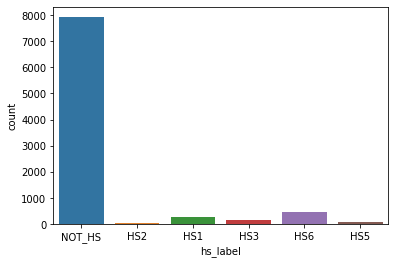
\includegraphics[width=\columnwidth, height=0.14\paperheight]{02.png}
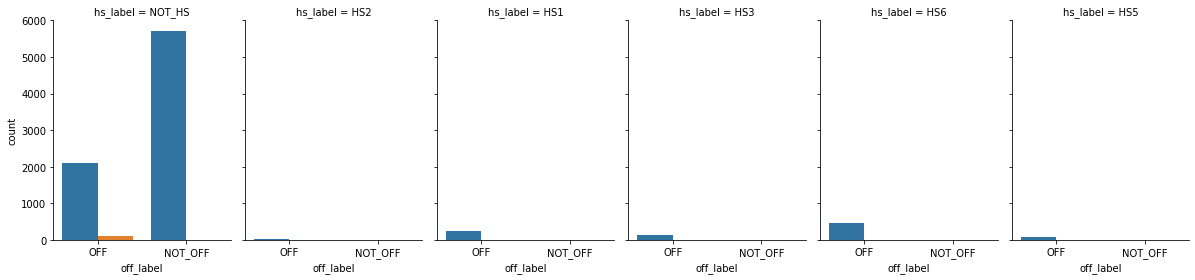
\includegraphics[width=\columnwidth, height=0.14\paperheight, scale=1.4]{03.png}

Then after applying the NLP aug, the data set was balanced in a reasonable manner.

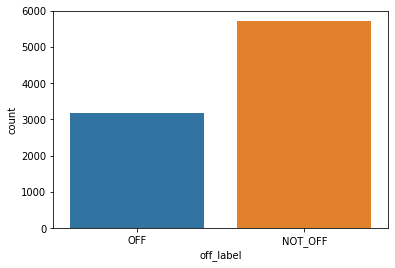
\includegraphics[width=\columnwidth, height=0.2\paperheight]{01.png}

The data set we have used we split it into 2 parts. First part is testing data which is 70\% of total number of the data set, and testing data which represents 30\% of the data set. Worth mentioning that the data set is from the \href{https://sites.google.com/view/arabichate2022/home}{competition}.


\end{document}
